\subsection{\cite{rebelo2011method}}
\label{sec:arebelo-domain-knowledge}
In this paper the authors discuss the use of domain knowledge in musical classification. In general the NoteEd project can't rely purely on standard musical conventions due to the potential mistakes which students are likely to make. 

However, the flow diagram reproduced in \cref{fig:arebelo-flow} which represents their musical extraction algorithm using domain knowledge provides an excellent reference for the order in which musical properties could be identified.
\begin{figure}[H]
  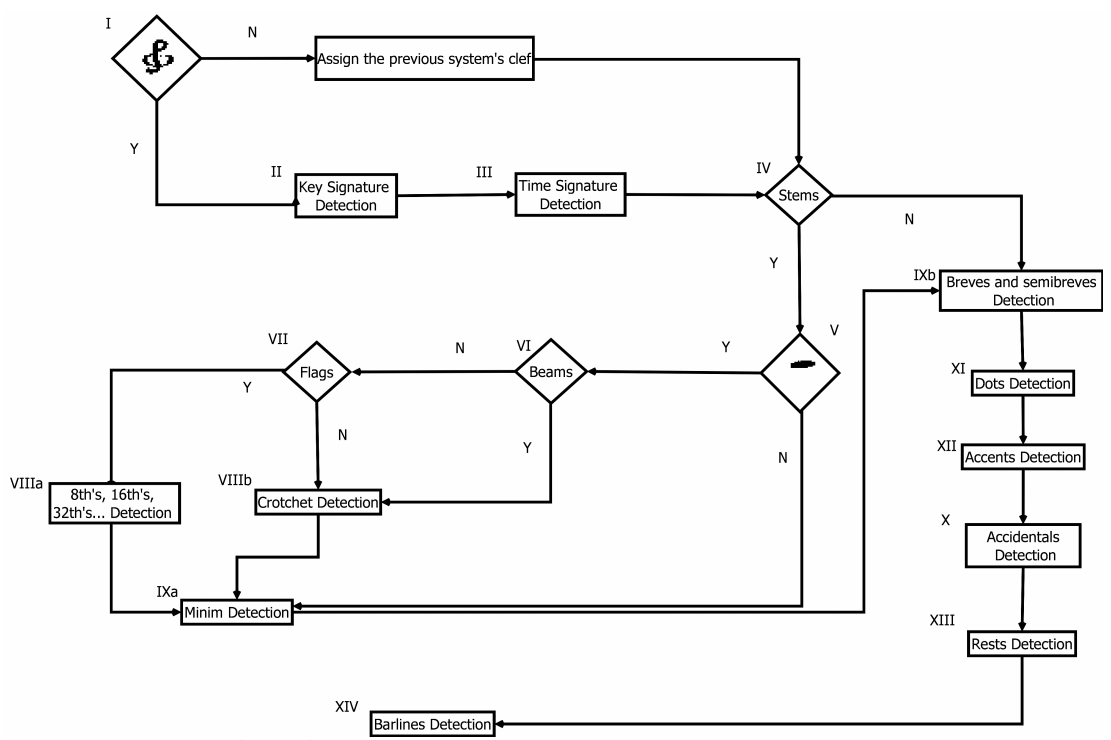
\includegraphics[width=\linewidth]{gfx/prior-research/arebelo-flow.png}
  \caption{Musical symbols extraction algorithm from \cite{rebelo2011method}}
  \label{fig:arebelo-flow}
\end{figure}
